\chapter{Gretl and Octave}
\label{chap:gretlOctave}

\section{Introduction}
\label{Octave-intro}

GNU \app{Octave}, written by John W. Eaton and others, is described as
``a high-level language, primarily intended for numerical
computations.''  The program is oriented towards ``solving linear and
nonlinear problems numerically'' and ``performing other numerical
experiments using a language that is mostly compatible with Matlab.''
(\url{www.gnu.org/software/octave}) \app{Octave} is available in
source-code form (naturally, for GNU software) and also in the form of
binary packages for MS Windows and Mac OS X.  Numerous contributed
packages that extend \app{Octave}'s functionality in various ways can
be found at \url{octave.sf.net}.


\section{\app{Octave} support in gretl}
\label{sec:Octave-support}

The support offered for \app{Octave} in gretl is similar to that
offered for \app{R} (chapter~\ref{chap:gretlR}).  For example, you can
open and edit \app{Octave} scripts in the gretl GUI.  Clicking
the ``execute'' icon in the editor window will send your code to
\app{Octave} for execution.  Figures~\ref{fig:Octedit} and
Figure~\ref{fig:Octout} show an \app{Octave} script and its output; in
this example we use the function \verb|logistic_regression| to
replicate some results from \cite{greene00}.

\begin{figure}[htbp]
  \centering
  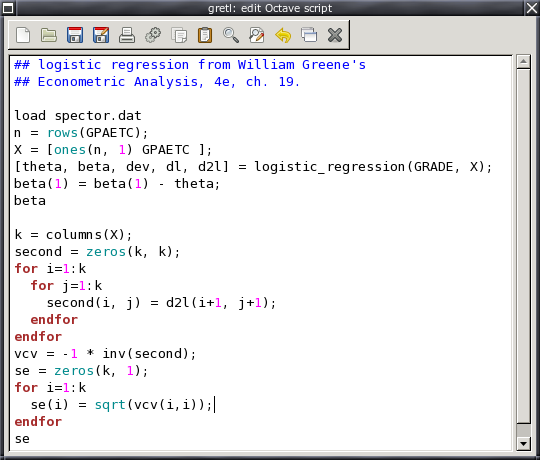
\includegraphics[scale=0.7]{figures/Octedit}
  \caption{\app{Octave} editing window}
  \label{fig:Octedit}
\end{figure}

\begin{figure}[htbp]
  \centering
  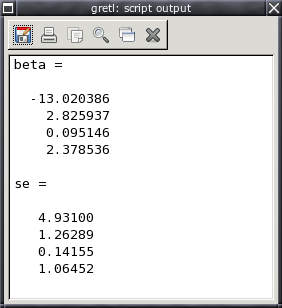
\includegraphics[scale=0.7]{figures/Octout}
  \caption{Output from \app{Octave}}
  \label{fig:Octout}
\end{figure}

In addition you can embed \app{Octave} code within a gretl script
using a \texttt{foreign} block, as described in connection with
\app{R}.  A trivial example is shown below: it simply loads and prints
the gretl data matrix within \app{Octave}, then takes it back to gretl
and checks for any difference (there should be none). (Note that in
\app{Octave}, appending ``\texttt{;}'' to a line suppresses verbose
output; leaving off the semicolon results in printing of the object
that is produced, if any.)
%
\begin{code}
open data4-1
matrix m = { dataset }
mwrite(m, "gretl.mat", 1)

foreign language=Octave
   gmat = gretl_loadmat("gretl.mat")
   gretl_export(gmat, "octave.mat")
end foreign

matrix chk = mread("octave.mat", 1)
eval maxr(maxc(abs(m - chk)))
\end{code}

The functions \texttt{gretl\_loadmat} and \texttt{gretl\_export},
which are predefined when you run \app{Octave} from within gretl, have
the following signatures:
\begin{code}
function A = gretl_loadmat(fname, autodot=1)

function gretl_export(X, fname, autodot=1)
\end{code}

By default traffic in matrices goes via the user's ``dotdir'' (see
section~\ref{sec:named-strings}) on the \app{Octave} side; that is,
the name of this directory is prepended to \texttt{filename} for both
reading and writing. (This is complementary to use of the
\textsl{export} and \textsl{import} parameters with gretl's
\texttt{mwrite} and \texttt{mread} functions, respectively.)  However,
if you wish to take control over the reading and writing locations you
can supply a zero value for \texttt{autodot} (or give an absolute
path) when calling \verb|gretl_loadmat| and \verb|gretl_export|: in
that case the \texttt{filename} argument is used as is.

\section{Illustration: spectral methods}
\label{sec:octave-coher}

We now present a more ambitious example which exploits \app{Octave}'s
handling of the frequency domain (and also its ability to use code
written for \app{MATLAB}), namely estimation of the spectral coherence
of two time series.  For this illustration we require two extra Octave
packages from \url{octave.sf.net}, namely those supporting spectral
functions (\texttt{specfun}) and signal processing (\texttt{signal}).
After downloading the packages you can install them from within
\app{Octave} as follows (using version numbers as of March 2010):
\begin{code}
pkg install specfun-1.0.8.tar.gz 
pkg install signal-1.0.10.tar.gz 
\end{code}

In addition we need some specialized \app{MATLAB} files made available
by Mario Forni of the University of Modena, at
\url{http://morgana.unimore.it/forni_mario/matlab.htm}. The files
needed are \texttt{coheren2.m}, \texttt{coheren.m}, \texttt{coher.m},
\texttt{cospec.m}, \texttt{crosscov.m}, \texttt{crosspec.m},
\texttt{crosspe.m} and \texttt{spec.m}. These are in a form appropriate
for MS Windows. On Linux you could run the following shell script
to get the files and remove the Windows end-of-file character (which
prevents the files from running under \app{Octave}):
\begin{code}
SITE=http://morgana.unimore.it/forni_mario/MYPROG
# download files and delete trailing Ctrl-Z
for f in \
  coheren2.m \
  coheren.m \
  coher.m \
  cospec.m \
  crosscov.m \
  crosspec.m \
  crosspe.m \
  spec.m ; do
    wget $SITE/$f && \
    cat $f | tr -d \\032 > tmp.m && mv tmp.m $f
done
\end{code}

The Forni files should be placed in some appropriate directory, and
you should tell \app{Octave} where to find them by adding that
directory to \app{Octave}'s \texttt{loadpath}. On Linux this can be
done via an entry in one's \verb|~/.octaverc| file. For example
\begin{code}
addpath("~/stats/octave/forni");
\end{code}
Alternatively, an \texttt{addpath} directive can be written into the
\app{Octave} script that calls on these files.

With everything set up on the \app{Octave} side we now write a gretl
script (see Listing~\ref{Octave-coher}) which opens a time-series
dataset, constructs and writes a matrix containing two series, and
defines a \texttt{foreign} block containing the \app{Octave}
statements needed to produce the spectral coherence matrix. This
matrix is exported via \verb|gretl_export| and picked up using
\texttt{mread}. Finally, we produce a graph from the matrix in gretl.
In the script this is sent to the screen; Figure~\ref{fig:coherence}
shows the same graph in PDF format.

\begin{script}[htbp]
  \caption{Estimation of spectral coherence via \app{Octave}}
  \label{Octave-coher}
\begin{scode}
open data9-7
matrix xy = { PRIME, UNEMP }
mwrite(xy, "xy.mat", 1)

foreign language=Octave
 pkg load signal
 # uncomment and modify the following if necessary
 # addpath("~/stats/octave/forni");
 xy = gretl_loadmat("xy.mat");
 x = xy(:,1);
 y = xy(:,2);
 # note: the last parameter is the Bartlett window size
 h = coher(x, y, 8);
 gretl_export(h, "h.mat");
end foreign

h = mread("h.mat", 1)
cnameset(h, "coherence")
gnuplot 1 --time-series --with-lines --matrix=h --output=display
\end{scode}
\end{script}

\begin{figure}[htbp]
  \centering
  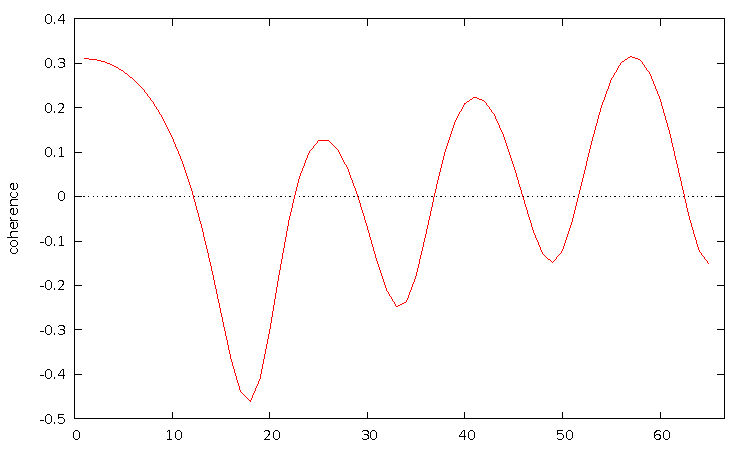
\includegraphics{figures/coherence}
  \caption{Spectral coherence estimated via \app{Octave}}
  \label{fig:coherence}
\end{figure}

%%% Local Variables: 
%%% mode: latex
%%% TeX-master: "gretl-guide"
%%% End: 

